\chapter{Introducción}
\pagenumbering{arabic}
\setcounter{page}{1}
%\renewcommand{\baselinestretch}{2} %doble espacio paratodo el texto
%\renewcommand{\baselinestretch }{1.5}
 


{\bf Ejemplo:}\par

En esta investigación se realizará la predicción de la respuesta correcta de una pregunta de opción múltiple, este tipo de pregunta de una evaluación requiere de conocimiento previo para ser respondida, mediante técnicas de aprendizaje no supervisado asociado con la experiencia previa. Como experiencia previa se usará las calificaciones anteriores obtenidas de los 2 últimos exámenes de los estudiantes.
\vskip 0.3cm
Para ello se plantea desarrollar un algoritmo de aprendizaje automático no supervisado llamado K-means, el cual sirve para crear clusters. Estos clusters se formarán con la data de las calificaciones  anteriores  de  los  estudiantes.Así  se  obtendría  un  valor  promedio,  Además,  se utilizará técnicas de estadísticas para crear un histograma de las opciones de las preguntas respondidas. Combinando estas 2 técnicas se obtendría un predicción por cada pregunta.
\vskip 0.3cm  
Este proyecto fue pensado debido a la problemática que se tiene al aplicar una evaluación y tener que esperar demasiado tiempo para obtener las respuestas correctas. Pero con lo que se desarrollara se obtendrá la respuesta correcta en corto tiempo.
\vskip 0.3cm 
Para cumplir los objetivos de este proyecto se tendrá primero que investigar acerca del aprendizaje automático no supervisado, así como las técnicas de estadísticas. Luego se desarrollará el algoritmo de aprendizaje automático no supervisado; ya hecho esto se procederá al desarrollo del prototipo de software web para poder ingresar los datos y hacer las pruebas. Finalmente se documentarán los resultados obtenidos.

\section{Justificación de la investigación}
La mayoría de las investigaciones se efectúan con un propósito definido. Tal propósito debe ser lo suficientemente fuerte para que justifique su realización. \cite{Erica}  

\begin{enumerate}
\item[(a)] Razones o motivos e importancia del tema a ser investigado. 
\item[(b)]Sustentar la pertinencia de la pregunta o problema que se abordará en la investigación.
\item[(c)]Considerar los resultados esperados e impactos previstos.
\end{enumerate}



{\bf Ejemplo:}\par

De esta forma, los sistemas integrados para el manejo, tratamiento y disposición final de los RSU que ya existen en diversas ciudades y capitales de los países desarrollados, se hacen referencias para la investigación y justifican posibles adaptaciones para la realidad peruana con el objetivo de que las ciudades sean ambientes más sustentables y competitivos.
\vskip 0.3cm
 Por lo tanto, se puede concluir que realmente existe una necesidad para planificar y modelar una red logística reversa que atienda a las necesidades de una región urbana y que contribuya con la adecuada disposición de los residuos urbanos. A partir del modelamiento es posible estructurar el sistema organizacional, gerencial, operacional y de información de toda la red  de logística reversa, y todas las otras acciones.


\section{Formulación del problema}

  En este trabajo, se propone responder a la siguiente pregunta:
 \begin{center} 
     ¿ Cómo predecir la respuesta correcta de una pregunta de opción múltiple?
 \end{center}


\section{Hipótesis}
Preferentemente para investigaciones explicativas debe ser una respuesta a priori y tentativa guardando coherencia con el problema científico, se formula como una proposición afirmativa, con un lenguaje claro y específico.  Las hipótesis se obtienen por deducción lógica y está sustentada en los conocimientos científicos. \par  
\vskip 0.3cm
{\bf Criterios para formular hipótesis:} \cite{Erica}
\begin{enumerate}
\item[a)] Toda hipótesis de investigación debe ser verificable estadísticamente.  Puede ser difícil o imposible de verificar porque no existe un conocimiento sobre el cual se pueda formular una hipótesis, o bien, porque una o más variables no son medibles.
\vskip 0.2cm
\item[b)] Toda hipótesis debe indicar la relación entre variables, lo que implica que las variables deben ser medibles.
\vskip 0.2cm
\item[c)] Toda hipótesis debe tener sus límites. Pueden escogerse hipótesis que sean sencillas de validar, y sin embargo, altamente significativas.
\vskip 0.2cm
\item[d)] El investigador debe tener una razón específica para considerar una hipótesis, ya sea teórica o por alguna evidencia concreta.    
\end{enumerate}





\section{Objetivos}
Es necesario establecer qué pretende la investigación, es decir, cuáles son sus objetivos. Hay investigaciones que buscan contribuir a resolver un problema en especial, y otras tienen como objetivo principal probar una teoría o aportar evidencia empírica en favor de ella. \par 
\vskip 0.3cm
Segun \cite{Rojas}, los objetivos tienen que expresarse con claridad para evitar posibles desviaciones en el proceso de investigación y deben ser susceptibles de alcanzarse; son las guías del estudio y hay que tenerlos presentes durante todo su desarrollo. Los objetivos deben ser congruentes entre sí.
\vskip 0.3cm
Describir el objetivo central o propósito del proyecto de investigación (debe estar alineado con el problema e hipótesis), así como los objetivos específicos, los cuales deben reflejar los cambios que se esperan lograr en trabajo de tesis (variables). Para estos objetivos específicos utilice verbos como: describir, indicar, modificar, controlar, producir (tecnologías), recuperar, etc..

\subsection{Generales}
\begin{enumerate}
\item[a)] Desarrollar un algoritmo de aprendizaje no supervisado para predecir la respuesta correcta de una pregunta de opción múltiple.
\end{enumerate}


\subsection{Específicos}
\begin{enumerate}
\item[a)] Codificar el algoritmo de aprendizaje no supervisado para trabajar con clusters.
\item[b)] Desarrollar del prototipo de software y aplicarla a la predicción de la respuesta correcta.
\item[c)] Realizar las pruebas y documentar resultados.
\end{enumerate}
\vskip 0.3cm


\section{Estructura de la tesis}

{\bf Ejemplo:}\par
\vskip 0.1cm
El presente trabajo está dividido en cinco capítulos. El primer capítulo presenta los aspectos generales del tema tratado: la formulación del problema, importancia de la investigación, los objetivos, además de la metodología de la investigación y la estructura de la tesis. En el segundo capítulo se contempla los conceptos de predicción, pregunta de opción múltiple y de prototipo de software.

El tercer capítulo trata del tema central de la tesis, diseñándose el algoritmo K-means, se muestra el proceso para hacer la predicción y como se desarrolló el prototipo de aplicación web.

En el cuarto capítulo se presentan los resultados obtenidos en la investigación. En el quinto capitulo se presentan las conclusiones, seguidas de las recomendaciones para futuras investigaciones relacionadas al tema en cuestión. 

Finalmente las referencias bibliográficas usadas para la investigación. Además de los apéndices donde se presentan el algoritmo elaborado, los datos de los resultados y los instrumentos usados para recoger información.

\chapter{Materiales y métodos}

{\bf Ejemplo:}\par

En este capítulo se explica cual fue la metodología empleada para la solución del problema formulado, además de una reseña del material bibliográfico investigado con relación a los temas considerados en esta investigación. Los conocimientos investigados son muy amplios, principalmente aquel que ayudó a consolidar las bases del conocimiento científico para elaborar esta tesis, como lo son los temas de optimización combinatoria, complejidad computacional, metaheurísticas, ciencia de la información y logística, conocimientos sin los cuales sería difícil de modelar y solucionar matemática y computacionalmente cualquier tipo de problema de optimización.
%\vskip 1cm 


\section{Marco teórico}
\subsection{Aprendizaje no supervisado}

\subsubsection{Definición}

Aprendizaje no supervisado es un método de aprendizaje automático donde un modelo esa justado  a  las  observaciones.  Se  distingue  del  aprendizaje  supervisado  por  el  hecho  de  que no hay un conocimiento a priori. En el aprendizaje no supervisado, un conjunto de datos de objetos de entrada es tratado. Así, el aprendizaje no supervisado típicamente trata los objetos de entrada como un conjunto de variables aleatorias, siendo construido un modelo de densidad para el conjunto de datos.
\vskip 1cm
En este método contamos con “objetos” o muestras que tiene un conjunto de características,de las que no sabemos a que clase o categoría pertenece, entonces la finalidad es el descubrimiento de grupos de “objetos” cuyas características afines nos permitan separar las diferentes clases \citep{Araujo}.

\subsubsection{Características}

En este apartado se muestran las principales características del método de aprendizaje no supervisadas \citep{Hinton_Sejnowski}.

\begin{itemize}
\item No necesitan de un profesor externo.
\item Muestran cierto grado de auto-organización.
\item La red descubre en los datos de entrada y de forma autónoma: características, regularidades, correlaciones y categorías.
\item Suelen requerir menores tiempos de entrenamiento que las supervisadas.
\item Abordan los siguientes tipos de problemas: familiaridad, análisis de componentes principales, agrupamiento y relación de características.
\end{itemize}

\subsubsection{Técnicas}

\begin{description}
	\item[Clustering] Agrupan objetos en regiones donde la similitud mutua es elevada.
	\item[Visualización] Permiten observar el espacio de instancias en un espacio de menor dimensión.
	\item[Reducción de la dimensionalidad] Los datos de entrada son agrupados en subespacios de una dimensión más baja que la inicial.
	\item[Extracción de características] construyen nuevos atributos (pocos) a partir de los atributos originales (muchos).
\end{description}


\subsection{Clustering}

Análisis de grupo o agrupamiento (en inglés, clustering) es un procedimiento de agrupación de una serie de vectores de acuerdo con un criterio. Esos criterios son por lo general distancia o similitud. La cercanía se define en términos de una determinada función de distancia, como la euclídea, aunque existen otras más robustas o que permiten extenderla a variables discretas. La medida más utilizada para medir la similitud entre los casos es la matriz de correlación entre los \( N x N \) casos. Sin embargo, también existen muchos algoritmos que se basan en la maximización de una propiedad estadística llamada verosimilitud \citep{Leonard_Peter}
\vskip 1cm
Generalmente, los vectores de un mismo grupo (o clústers) comparten propiedades comunes. El conocimiento de los grupos puede permitir una descripción sintética de un conjunto de datos multidimensional complejo. De ahí su uso en minería de datos. Esta descripción sintética se consigue sustituyendo el detalle de todos los elementos de un grupo por la de un representante característico del mismo.

\begin{figure}[ht]
	\begin{center}
		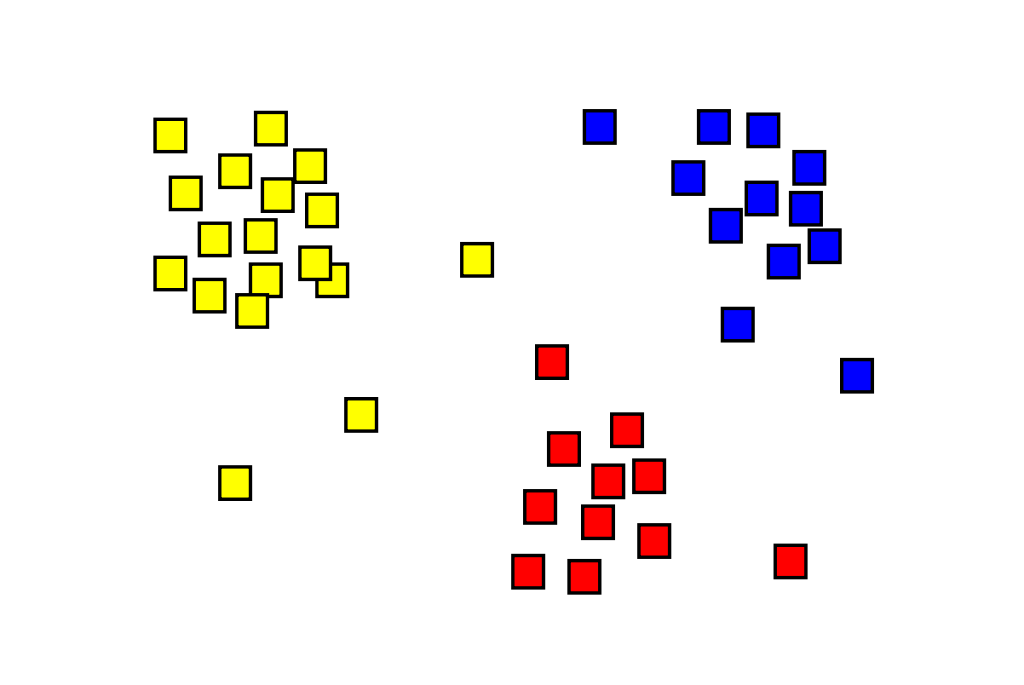
\includegraphics[width=0.3\textwidth]{clustering}
	\end{center}
	\begin{center}
		\vskip -0.5cm
		\caption{\small{El resultado de un análisis de grupo, mostrado como la coloración de cuadrados en tres grupos.}}
		{\small{Fuente: }}
	\end{center}
\end{figure}

Clustering es considerado una técnica de aprendizaje no supervisado puesto que busca encontrar relaciones entre variables descriptivas pero no la que guardan con respecto a una variable objetivo.


\subsubsection{Técnicas de clustering}

Existen dos grandes técnicas para el agrupamiento de casos:

\begin{itemize}
	\item Agrupamiento jerárquico, que puede ser aglomerativo o divisivo.
	\item Agrupamiento no jerárquico, en los que el número de grupos se determina de antemano y las observaciones se van asignando a los grupos en función de su cercanía. Existen los métodos de K-means y K-medoid.

\end{itemize}

\subsubsection{Algoritmos}

Existen diversas implementaciones de algoritmos concretos. Por ejemplo, el de las K-mediaso K-means. Es uno de los más antiguos pero su uso es muy extendido en la actualidad.
\vskip 1cm
El algoritmo de K-means es un algoritmo particional y fue propuesto en los ’50. El algoritmo intenta encontrar una partición de nuestros ejemplos en \(K\) agrupaciones, de forma que cada ejemplo pertenezca a una de ellas, concretamente a aquella cuyo centro geométrico esté más cerca. El mejor valor de \(K\) para que la clasificación separe lo mejor posible los ejemplos no se conoce a priori, y depende completamente de los datos con los que trabajemos \citep{Jain}
\vskip 1cm 
A pesar de que su primera aparición es desde hace más de 50 años sigue siendo de los algoritmos más utilizados para clustering por su facilidad de implementación, simpleza y buenos resultados empíricos.
\vskip 1cm 

\textbf{Los principales pasos del algoritmo son los siguientes:}

\begin{enumerate}
	\item Seleccionar una partición inicial (determinada por los centros de los clusters) con \(K\) clus-ters, repetir los pasos 2 y 3 hasta que los clusters se lleguen a estabilizar.
	\item Generar una nueva partición asignando cada dato al cluster cuyo centro está más cercano.	
	\item Calcular los nuevos centros de los clusters \(c(1)....c(K)\) (promediando los datos asignados a ese cluster en el paso anterior si la distancia es la euclídea).
\end{enumerate}

\textbf{El algoritmo K-medias requiere del usuario los siguientes parámetros:}

\begin{itemize}
	\item Número de clusters.
	\item Inicialización de los clusters (centros).
	\item Distancia (en general la distancia euclídea).
\end{itemize}

\begin{figure}[ht]
	\begin{center}
		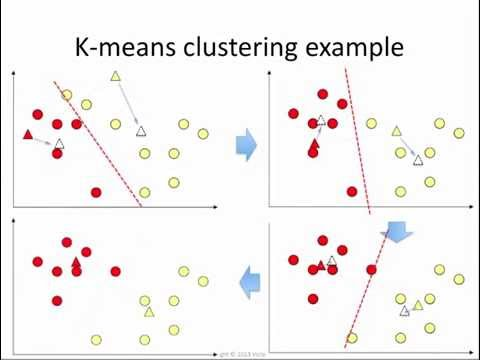
\includegraphics[width=0.8\textwidth]{proceso_kmeans}
	\end{center}
	\begin{center}
		\vskip -0.5cm
		\caption{\small{Proceso K-means.}}
		{\small{Fuente: }}
	\end{center}
\end{figure}












\subsubsection{Algoritmos de clustering}

\subsection{Probabilidad}

\subsubsection{Definición}
\subsubsection{Técnicas}
\subsubsection{Teoría de bayes}

\subsection{Aprendizaje no supervisado}

\subsubsection{Definición}
\subsubsection{Ventajas}
\subsubsection{Aplicación web}
\subsubsection{LAMP}
\subsubsection{Software}







\subsection{Optimización combinatoria y complejidad computacional}
\subsubsection{Problemas combinatorios}
\subsubsection{Heurísticas y metaheurísticas}

\subsection{Sustentabilidad}

{\bf Ejemplo:}\par

La configuración, característica, jurisdicción administrativa, relaciones económicas, sociales y ambientales de un espacio urbano se define por la población y por la función que ella desarrolla en un área geográfica o región \citep{Bugliarello}. De este modo las ciudades son sistemas dinámicos que interactúan continua y constantemente con su medio ambiente, acompañando las características, perfil, cultura y ritmo de desarrollo económico y social de su población. Los medios de transporte juegan un papel importante en tal ritmo de desarrollo de las ciudades, ya que ellos tienen como función relacional los factores poblacionales con los factores uso del suelo.  
\vskip 1cm
El desarrollo sustentable, (Figura 2.1), estará garantizado si se consideran tres aspectos fundamentales: económico, social y ambiental, donde la intersección de estos aspectos garantiza la calidad de vida en el espacio urbano y el equilibrio en las clases sociales en busca del bienestar \citep{Tanguay}.

\begin{figure}[ht]
\begin{center}
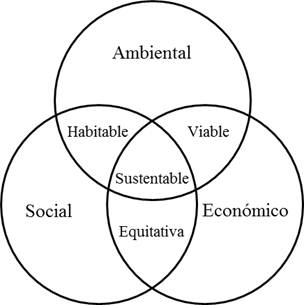
\includegraphics[width=0.3\textwidth]{Figura2}
\end{center}
\begin{center}
\vskip -0.5cm
\caption{\small{Aspectos claves para el desarrollo sustentable.}}
{\small{Fuente: \cite{Tanguay}}}
\end{center}
\end{figure}

\subsection{Logística directa y reversa}

\subsubsection{Logística directa}

{\bf Ejemplo:}\par

\cite{Ghiani} entienden que la logística trata de la planificación y control de los flujos de materiales e informaciones relacionadas en las organizaciones, tanto en los sectores público y privado. Además su misión es hacer la entrega de los productos correctos, en el local correcto y en la hora correcta, optimizando los costos operacionales totales del proceso.
satisfaciendo un determinado conjunto de restricciones o condiciones.\par

\subsubsection{Logística reversa}

{\bf Ejemplo:}\par

En los años 90 se presentaron definiciones generales las cuales vienen siendo mejoradas. \cite{Dekker} presenta una mejora en la definición de logística reversa como  ”el proceso de planificación, implementación y control de los flujos de materias-primas, en procesos de inventarios y bienes acabados, desde el punto de fabricación, distribución o uso, hacia el punto de recuperación o de eliminación”. 
\begin{figure}[ht]
\begin{center}
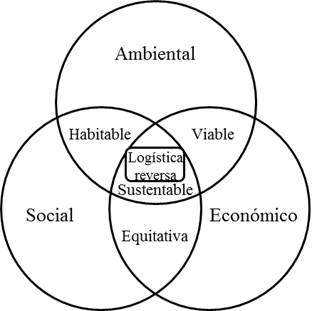
\includegraphics[width=0.3\textwidth]{Figura1}
\end{center}
\begin{center}
\vskip -0.5cm
\caption{\small{Logística reversa incluida en el desarrollo sustentable.}}
{\small{Fuente: Adaptación de \cite{Tanguay}}}
\end{center}
\end{figure}


\subsubsection{Modelos}

\subsection{Modelamiento y ruteo }

{\bf Ejemplo:}\par

El modelamiento matemático es una alternativa para expresar formalmente hechos reales que pueden ayudar en el proceso de toma de decisiones. El modelamiento permite la simulación de procesos  y de escenarios con la introducción de índices de desempeño que permitan cuantificar los costos y beneficios de la implementación del sistema, la mejoría de la sustentabilidad urbana y por supuesto los índices de contaminación en las grandes ciudades y su impacto en todo el medio ambiente. 

\subsubsection{Modelos utilizados en los problemas de ruteo de vehículo }

{\bf Ejemplo:}\par

El problema de ruteo de vehículos \citep{Ombuki, Yeun} y sus variantes han ganado mucho interés en la comunidad académica. La intención de estar más cerca a la realidad mediante el modelamiento matemático, hace que se hayan desarrollado nuevos modelos de optimización. \par
\vskip 0.2cm

\begin{table}[h!]
\begin{center}
\caption{\small{Resultados computacionales obtenidos en el modelo de \cite{Ombuki}}}
\end{center}
\vskip -0.7cm
\begin{tabular}{|c|c|c|c|c|}
\hline 
\rowcolor{LightBlue2}{\small Escenarios} & {\small Demanda cliente (ton.)} & {\small Tiempo (min.)} & {\small Costo ($\$$)} \\ 
\hline 
{\small 1} & {\small P1:1; P2:2; P3:2; P4:2; P5:1} & {\small 0.12} & {\small 667.42} \\ 
\hline 
{\small 2} & {\small P1:1; P2:2; P3:2; P4:2; P5:1; P:4; P7:3} & {\small 56.54} & {\small 1744.35} \\ 
\hline 
{\small 3} & {\small P1: 1; P2:2; P3:2; P4:2; P5:1; P6: 4; P7:3; P8:2; P9:2} & {\small 287.70} & {\small 1750.72} \\ 
\hline 
{\small 4} & {\small P1:1; P2:2; P3: 2; P4:2; P5:1; P6:4; P7:3; P8:2; P9:2; P10:1} & {\small 1848.57} & {\small 1773.46} \\ 
\hline 
{\small 5} & {\small P1:1; P2:2; P3: 2; P4:2; P5:1; P6:4; P7:3; P8:2; P9:2; P10:1} & {\small 1848.57} & {\small 1773.46} \\ 
\hline 
{\small 6} & {\small P1:1; P2:2; P3: 2; P4:2; P5:1; P6:4; P7:3; P8:2; P9:2; P10:1} & {\small 1848.57} & {\small 1773.46} \\ 
\hline 
\end{tabular} 
\begin{center}
\vskip -0.2cm
{\small{Fuente: Resultados obtenidos con CPLEX.}}
\end{center}
\end{table}



\section{Método de la investigación}
De acuerdo con \cite{Erica}, para el desarrollo del método debe presentarse un bosquejo de la manera  en que se propone llevar a cabo la investigación, es decir, el camino a seguir o los pasos a seguir para realizar una cosa. Cuando mas complejo sea el bosquejo  más fácil se desarrollará el proceso de investigación. Se utiliza el vocablo método en vez de metodología, ya este último se considera equivocado, en el sentido en que se le utiliza comúnmente en informes de investigación. 
\vskip 0.3cm
Los tipos de método a usar para TG en informática se considera:
\begin{enumerate}
\item[a)] {\bf Método deductivo:} Es un método de razonamiento que consiste en tomar conclusiones generales para explicaciones partículares. El método se inicia con el análisis de los postulados, teoremas, leyes, principios, etc., de aplicación universal y de comprobada validez, para aplicarlos  a soluciones o hechos particulares. 

\item[b)]{\bf Método cuantitativo:} Se fundamenta en la medición de las características de los fenómenos, lo cual supone derivar de un marco conceptual pertinente al problema analizado, una serie de postulados que expresen relaciones entre las variables estudiadas de forma deductiva, es decir, estudia fenómenos susceptibles de cuantificación y utiliza pruebas estadísticas para el análisis de datos. Este método tiende a generalizar y normalizar resultados. 
\end{enumerate}

Por lo tanto, plantear el objeto de estudio, el diseño de investigación a usar, las técnicas de recolección de la información a ser utilizadas, definir la población y tamaño de la muestra que debe ser representativa y necesaria para hacer generalizaciones, {\bf etapas del estudio} y análisis estadístico. El método de estudio entre otras cosas se refiere a la secuencia de pasos que se sigue para alcanzar los objetivos trazados, considerando los métodos deductivo y cuantitativo.\par




\chapter{Nombre de la propuesta o tema central de la tesis}

{\bf Ejemplo:}\par

Basado en los conceptos discutidos en los capítulos 1 y 2, así como de la experiencia obtenida del análisis de resultados de los modelos matemáticos estudiados y programados con CPLEX, se caracterizan los principales elementos que componen el modelo propuesto en este trabajo para la colecta y transporte de RSU en un área urbana. Así, se estructura una red logística reversa para los RSU considerando diferentes centros especializados o unidades  productivas para atender las diferentes fases del proceso en la red. En este proceso de modelamiento se tuvo cuidado en mantener la propuesta lo mas cerca a la realidad de las ciudades, donde el modelo fue testado y validado.

\section{Proceso de modelamiento} 

{\bf Ejemplo:}\par

La planificación y modelamiento del sistema de logística reversa de una área urbana es una fase importante y estratégica, para obtener en el futuro óptimos resultados en el proceso de gerenciamiento y operación del sistema reverso de RSU. El modelamiento permite determinar la localización de las estaciones de colecta y de unidades especiales necesarias, asi como el flujo que será movido a los largo de la red permitiendo dimensionar todo el sistema y sus componentes (Figura 3.1).
\vskip 0.3cm
\begin{figure}[ht]
\begin{center}
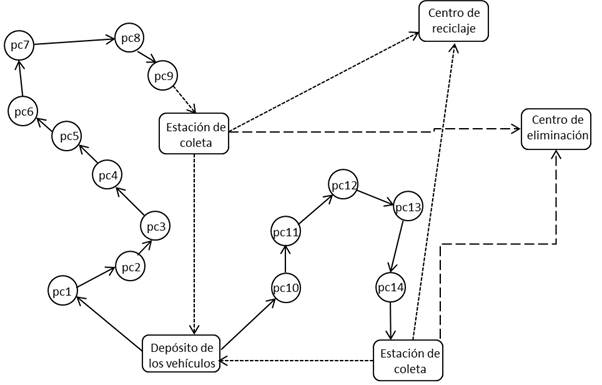
\includegraphics[width=.6\textwidth]{Figura3}
\end{center}
\begin{center}
\vskip -0.5cm
\caption{\small{Esquema del proceso de colecta y transporte de RSU.}}
{\small{Fuente: Elaboración propia}}
\end{center}
\end{figure}

\subsection{Proceso de ruteo}

\begin{algorithm}
\begin{algorithmic}[htbp]
\REQUIRE NP,NV,Dij,Tij,DM,CM,P,numVecinos,numIteraciones,persistencia.  % Entrada
 \label{lin:algoritmo_pseudocodigo}
\ENSURE RUTAS.                                                          % Salida

\STATE $i \leftarrow 0 $

\STATE Inicializar lista de vecinos y la memoria tabú.
\STATE Generar solución inicial.
\STATE Evaluar solucion inicial.
\WHILE {$numIteraciones  >  i$}
\STATE Generar los vecinos.
\STATE Evaluar los vecinos.
\STATE Elegir al mejor vecino.
\IF{Mejor vecino tiene una mejor solución}
\STATE Reemplazar solución inicial y agregarlo a la memoria tabú con su persistencia respectiva.

\ELSE
\STATE Agregar mejor vecino a la memoria tabú con su persistencia respectiva.

\ENDIF
\STATE Disminuir persistencia de todos los que estan en la memoria tabú excepto del último elemento agregado.

\IF{La persistencia de los elementos llega a cero}
\STATE Retirar el elemento de la memoria tabú.
\ENDIF

\STATE $i++$
\ENDWHILE
\RETURN  La mejor solución.


\end{algorithmic}
\caption{Busca tabú}
\label{alg:algoritmoBT}
\end{algorithm}


\section{Implementación} 



\chapter{Resultados y discusión de la tesis}


Al culminar con la investigación se llegaron a resultados interesantes del punto de vista tanto teórico como computacional. Estos resultados muestran que se contrasta la hipótesis planteada durante el proceso de elaboración del plan de investigación, es decir, que se logró demostrar la relación entre las variables de estudio formuladas en la investigación.

\section{Teóricos}

\section{Computacionales}




\chapter{Consideraciones finales}


\section{Conclusiones}

{\bf Ejemplo}\\
La investigación bibliográfica revela que realmente existe una preocupación de los gobiernos con el destino final de los residuos sólidos, con el objetivo de preservar la salud de la población y el medio ambiente urbano y rural. Por ejemplo, se observa la creación de la Ley 12305. Sin embargo existe una laguna entre las metas propuestas en la ley con las metas reales de los gobiernos locales. Eso se debe a la falta de una buena estructura organizacional, gerencial y operacional de los gobiernos locales capaz de atender las demandas locales y las necesidades de la población.
\vskip 0.3cm
La falta de cuadros especializados, tanto en los gobiernos centrales como locales, para realizar la planificación y modelamiento de una red logística reversa puede ser compensada con la contribución de los investigadores que actúan en ese campo del conocimiento. Es muy difícil la formación de un equipo que tenga todo el conocimiento en las áreas de ciencia de la computación, de geo procesamiento, de modelamiento matemático y de logística reversa, entre otras. Esa es una de las principales justificativas que los gobiernos, argumentan a la falta de planificación de una red logística reversa que funciones eficaz y eficientemente. 
\vskip 0.3cm
Por lo tanto, como quedó demostrado a lo largo de este trabajo, es posible realizar el modelamiento matemático para este tipo de problema con baja inversión, así como aplicarlo en varias regiones sin necesidad de grandes cambios en el modelamiento propuesto. El modelo propuesto calcula los flujos en la red logística reversa, permitiendo dimensionar la cantidad y capacidad de las unidades productivas y de los vehículos. 
\vskip 0.3cm
...


\section{Trabajos futuros}



\cleardoublepage
\addcontentsline{toc}{chapter}{Bibliografía}
\bibliographystyle{apalike}  % estilo de la bibliografía APA.
\bibliography{Bibliografia}   % Bibliografia.bib es el fichero donde está salvada la bibliografía.


